\hypertarget{S3Classes_8h}{
\section{S3Classes.h File Reference}
\label{S3Classes_8h}\index{S3Classes.h@{S3Classes.h}}
}


This graph shows which files directly or indirectly include this file:\begin{figure}[H]
\begin{center}
\leavevmode
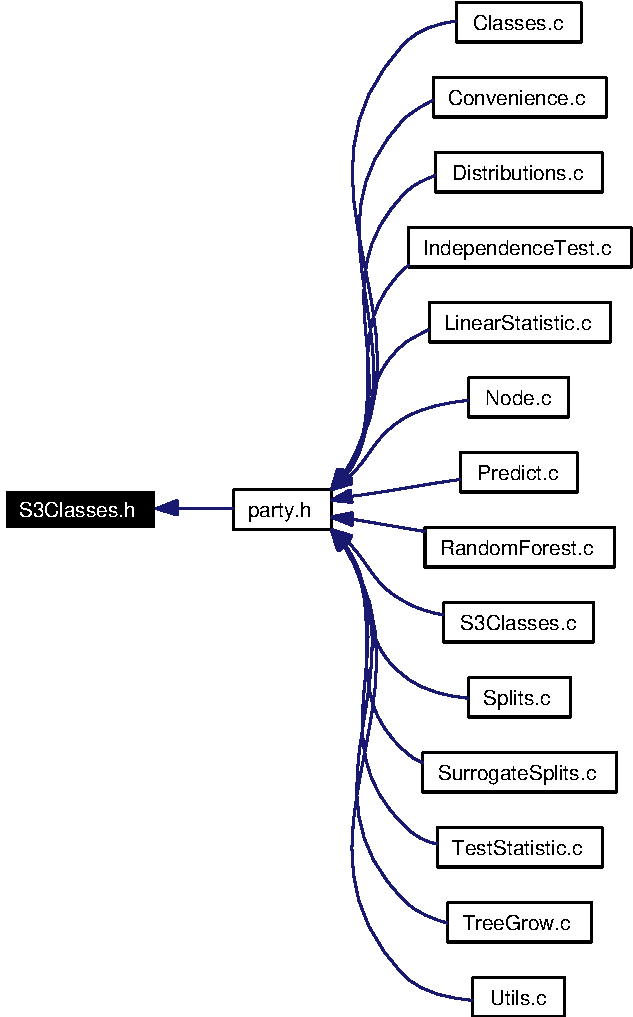
\includegraphics[width=168pt]{S3Classes_8h__dep__incl}
\end{center}
\end{figure}
\subsection*{Functions}
\begin{CompactItemize}
\item 
void \hyperlink{S3Classes_8h_a0}{C\_\-init\_\-node} (SEXP node, int nobs, int ninputs, int nsurr, int q)
\item 
void \hyperlink{S3Classes_8h_a1}{S3set\_\-node\-ID} (SEXP node, int node\-ID)
\item 
int \hyperlink{S3Classes_8h_a2}{S3get\_\-node\-ID} (SEXP node)
\item 
SEXP \hyperlink{S3Classes_8h_a3}{S3get\_\-nodeweights} (SEXP node)
\item 
SEXP \hyperlink{S3Classes_8h_a4}{S3get\_\-teststat} (SEXP node)
\item 
SEXP \hyperlink{S3Classes_8h_a5}{S3get\_\-criterion} (SEXP node)
\item 
SEXP \hyperlink{S3Classes_8h_a6}{S3get\_\-maxcriterion} (SEXP node)
\item 
void \hyperlink{S3Classes_8h_a7}{S3set\_\-nodeterminal} (SEXP node)
\item 
int \hyperlink{S3Classes_8h_a8}{S3get\_\-nodeterminal} (SEXP node)
\item 
SEXP \hyperlink{S3Classes_8h_a9}{S3get\_\-primarysplit} (SEXP node)
\item 
SEXP \hyperlink{S3Classes_8h_a10}{S3get\_\-surrogatesplits} (SEXP node)
\item 
SEXP \hyperlink{S3Classes_8h_a11}{S3get\_\-prediction} (SEXP node)
\item 
void \hyperlink{S3Classes_8h_a12}{C\_\-init\_\-orderedsplit} (SEXP split, int nobs)
\item 
void \hyperlink{S3Classes_8h_a13}{C\_\-init\_\-nominalsplit} (SEXP split, int nlevels, int nobs)
\item 
void \hyperlink{S3Classes_8h_a14}{S3set\_\-variable\-ID} (SEXP split, int variable\-ID)
\item 
int \hyperlink{S3Classes_8h_a15}{S3get\_\-variable\-ID} (SEXP split)
\item 
int \hyperlink{S3Classes_8h_a16}{S3is\_\-ordered} (SEXP split)
\item 
void \hyperlink{S3Classes_8h_a17}{S3set\_\-ordered} (SEXP split)
\item 
void \hyperlink{S3Classes_8h_a18}{S3set\_\-nominal} (SEXP split)
\item 
SEXP \hyperlink{S3Classes_8h_a19}{S3get\_\-splitpoint} (SEXP split)
\item 
SEXP \hyperlink{S3Classes_8h_a20}{S3get\_\-splitstatistics} (SEXP split)
\item 
SEXP \hyperlink{S3Classes_8h_a21}{S3get\_\-leftnode} (SEXP node)
\item 
SEXP \hyperlink{S3Classes_8h_a22}{S3get\_\-rightnode} (SEXP node)
\item 
SEXP \hyperlink{S3Classes_8h_a23}{S3get\_\-table} (SEXP node)
\item 
int \hyperlink{S3Classes_8h_a24}{S3get\_\-toleft} (SEXP split)
\item 
void \hyperlink{S3Classes_8h_a25}{S3set\_\-toleft} (SEXP split, int left)
\end{CompactItemize}


\subsection{Function Documentation}
\hypertarget{S3Classes_8h_a0}{
\index{S3Classes.h@{S3Classes.h}!C_init_node@{C\_\-init\_\-node}}
\index{C_init_node@{C\_\-init\_\-node}!S3Classes.h@{S3Classes.h}}
\subsubsection[C\_\-init\_\-node]{\setlength{\rightskip}{0pt plus 5cm}void C\_\-init\_\-node (SEXP {\em node}, int {\em nobs}, int {\em ninputs}, int {\em nsurr}, int {\em q})}}
\label{S3Classes_8h_a0}




Definition at line 11 of file S3Classes.c.

References CRITERION\_\-LENGTH, NODE\_\-LENGTH, S3\_\-CRITERION, S3\_\-i\-CRITERION, S3\_\-MAXCRITERION, S3\_\-NODEID, S3\_\-PREDICTION, S3\_\-PSPLIT, S3\_\-SSPLIT, S3\_\-STATISTICS, S3\_\-TERMINAL, S3\_\-WEIGHTS, and SPLIT\_\-LENGTH.

Referenced by C\_\-splitnode(), R\_\-Ensemble(), R\_\-Node(), and R\_\-Tree\-Grow().\hypertarget{S3Classes_8h_a13}{
\index{S3Classes.h@{S3Classes.h}!C_init_nominalsplit@{C\_\-init\_\-nominalsplit}}
\index{C_init_nominalsplit@{C\_\-init\_\-nominalsplit}!S3Classes.h@{S3Classes.h}}
\subsubsection[C\_\-init\_\-nominalsplit]{\setlength{\rightskip}{0pt plus 5cm}void C\_\-init\_\-nominalsplit (SEXP {\em split}, int {\em nlevels}, int {\em nobs})}}
\label{S3Classes_8h_a13}




Definition at line 123 of file S3Classes.c.

References S3\_\-ORDERED, S3\_\-SPLITPOINT, S3\_\-SPLITSTATISTICS, S3\_\-TABLE, S3\_\-TOLEFT, S3\_\-VARIABLEID, and SPLIT\_\-LENGTH.

Referenced by C\_\-Node().\hypertarget{S3Classes_8h_a12}{
\index{S3Classes.h@{S3Classes.h}!C_init_orderedsplit@{C\_\-init\_\-orderedsplit}}
\index{C_init_orderedsplit@{C\_\-init\_\-orderedsplit}!S3Classes.h@{S3Classes.h}}
\subsubsection[C\_\-init\_\-orderedsplit]{\setlength{\rightskip}{0pt plus 5cm}void C\_\-init\_\-orderedsplit (SEXP {\em split}, int {\em nobs})}}
\label{S3Classes_8h_a12}




Definition at line 99 of file S3Classes.c.

References S3\_\-ORDERED, S3\_\-SPLITPOINT, S3\_\-SPLITSTATISTICS, S3\_\-TABLE, S3\_\-TOLEFT, S3\_\-VARIABLEID, and SPLIT\_\-LENGTH.

Referenced by C\_\-Node(), and C\_\-surrogates().\hypertarget{S3Classes_8h_a5}{
\index{S3Classes.h@{S3Classes.h}!S3get_criterion@{S3get\_\-criterion}}
\index{S3get_criterion@{S3get\_\-criterion}!S3Classes.h@{S3Classes.h}}
\subsubsection[S3get\_\-criterion]{\setlength{\rightskip}{0pt plus 5cm}SEXP S3get\_\-criterion (SEXP {\em node})}}
\label{S3Classes_8h_a5}




Definition at line 63 of file S3Classes.c.

References S3\_\-CRITERION, and S3\_\-i\-CRITERION.

Referenced by C\_\-Node().\hypertarget{S3Classes_8h_a21}{
\index{S3Classes.h@{S3Classes.h}!S3get_leftnode@{S3get\_\-leftnode}}
\index{S3get_leftnode@{S3get\_\-leftnode}!S3Classes.h@{S3Classes.h}}
\subsubsection[S3get\_\-leftnode]{\setlength{\rightskip}{0pt plus 5cm}SEXP S3get\_\-leftnode (SEXP {\em node})}}
\label{S3Classes_8h_a21}




Definition at line 91 of file S3Classes.c.

References S3\_\-LEFT.

Referenced by C\_\-get\_\-node(), C\_\-get\_\-nodebynum(), C\_\-splitsurrogate(), and C\_\-Tree\-Grow().\hypertarget{S3Classes_8h_a6}{
\index{S3Classes.h@{S3Classes.h}!S3get_maxcriterion@{S3get\_\-maxcriterion}}
\index{S3get_maxcriterion@{S3get\_\-maxcriterion}!S3Classes.h@{S3Classes.h}}
\subsubsection[S3get\_\-maxcriterion]{\setlength{\rightskip}{0pt plus 5cm}SEXP S3get\_\-maxcriterion (SEXP {\em node})}}
\label{S3Classes_8h_a6}




Definition at line 67 of file S3Classes.c.

References S3\_\-CRITERION, and S3\_\-MAXCRITERION.

Referenced by C\_\-get\_\-node(), and C\_\-Node().\hypertarget{S3Classes_8h_a2}{
\index{S3Classes.h@{S3Classes.h}!S3get_nodeID@{S3get\_\-nodeID}}
\index{S3get_nodeID@{S3get\_\-nodeID}!S3Classes.h@{S3Classes.h}}
\subsubsection[S3get\_\-nodeID]{\setlength{\rightskip}{0pt plus 5cm}int S3get\_\-node\-ID (SEXP {\em node})}}
\label{S3Classes_8h_a2}




Definition at line 46 of file S3Classes.c.

References S3\_\-NODEID.

Referenced by C\_\-get\_\-nodebynum(), and C\_\-get\_\-node\-ID().\hypertarget{S3Classes_8h_a8}{
\index{S3Classes.h@{S3Classes.h}!S3get_nodeterminal@{S3get\_\-nodeterminal}}
\index{S3get_nodeterminal@{S3get\_\-nodeterminal}!S3Classes.h@{S3Classes.h}}
\subsubsection[S3get\_\-nodeterminal]{\setlength{\rightskip}{0pt plus 5cm}int S3get\_\-nodeterminal (SEXP {\em node})}}
\label{S3Classes_8h_a8}




Definition at line 75 of file S3Classes.c.

References S3\_\-TERMINAL.

Referenced by C\_\-get\_\-node(), C\_\-get\_\-nodebynum(), and C\_\-Tree\-Grow().\hypertarget{S3Classes_8h_a3}{
\index{S3Classes.h@{S3Classes.h}!S3get_nodeweights@{S3get\_\-nodeweights}}
\index{S3get_nodeweights@{S3get\_\-nodeweights}!S3Classes.h@{S3Classes.h}}
\subsubsection[S3get\_\-nodeweights]{\setlength{\rightskip}{0pt plus 5cm}SEXP S3get\_\-nodeweights (SEXP {\em node})}}
\label{S3Classes_8h_a3}




Definition at line 50 of file S3Classes.c.

References S3\_\-WEIGHTS.

Referenced by C\_\-get\_\-node(), C\_\-get\_\-nodeweights(), C\_\-getweights(), C\_\-splitnode(), C\_\-splitsurrogate(), C\_\-surrogates(), C\_\-Tree\-Grow(), R\_\-Ensemble(), R\_\-predict\-RF(), R\_\-predict\-RF2(), R\_\-predict\-RF\_\-weights(), and R\_\-Tree\-Grow().\hypertarget{S3Classes_8h_a11}{
\index{S3Classes.h@{S3Classes.h}!S3get_prediction@{S3get\_\-prediction}}
\index{S3get_prediction@{S3get\_\-prediction}!S3Classes.h@{S3Classes.h}}
\subsubsection[S3get\_\-prediction]{\setlength{\rightskip}{0pt plus 5cm}SEXP S3get\_\-prediction (SEXP {\em node})}}
\label{S3Classes_8h_a11}




Definition at line 87 of file S3Classes.c.

References S3\_\-PREDICTION.

Referenced by C\_\-get\_\-prediction(), C\_\-getpredictions(), C\_\-Node(), R\_\-predict\-RF(), and R\_\-predict\-RF\_\-weights().\hypertarget{S3Classes_8h_a9}{
\index{S3Classes.h@{S3Classes.h}!S3get_primarysplit@{S3get\_\-primarysplit}}
\index{S3get_primarysplit@{S3get\_\-primarysplit}!S3Classes.h@{S3Classes.h}}
\subsubsection[S3get\_\-primarysplit]{\setlength{\rightskip}{0pt plus 5cm}SEXP S3get\_\-primarysplit (SEXP {\em node})}}
\label{S3Classes_8h_a9}




Definition at line 79 of file S3Classes.c.

References S3\_\-PSPLIT.

Referenced by C\_\-get\_\-node(), C\_\-Node(), C\_\-splitnode(), C\_\-splitsurrogate(), and C\_\-surrogates().\hypertarget{S3Classes_8h_a22}{
\index{S3Classes.h@{S3Classes.h}!S3get_rightnode@{S3get\_\-rightnode}}
\index{S3get_rightnode@{S3get\_\-rightnode}!S3Classes.h@{S3Classes.h}}
\subsubsection[S3get\_\-rightnode]{\setlength{\rightskip}{0pt plus 5cm}SEXP S3get\_\-rightnode (SEXP {\em node})}}
\label{S3Classes_8h_a22}




Definition at line 95 of file S3Classes.c.

References S3\_\-RIGHT.

Referenced by C\_\-get\_\-node(), C\_\-get\_\-nodebynum(), C\_\-splitsurrogate(), and C\_\-Tree\-Grow().\hypertarget{S3Classes_8h_a19}{
\index{S3Classes.h@{S3Classes.h}!S3get_splitpoint@{S3get\_\-splitpoint}}
\index{S3get_splitpoint@{S3get\_\-splitpoint}!S3Classes.h@{S3Classes.h}}
\subsubsection[S3get\_\-splitpoint]{\setlength{\rightskip}{0pt plus 5cm}SEXP S3get\_\-splitpoint (SEXP {\em split})}}
\label{S3Classes_8h_a19}




Definition at line 174 of file S3Classes.c.

References S3\_\-SPLITPOINT.

Referenced by C\_\-get\_\-node(), C\_\-Node(), C\_\-splitnode(), C\_\-splitsurrogate(), and C\_\-surrogates().\hypertarget{S3Classes_8h_a20}{
\index{S3Classes.h@{S3Classes.h}!S3get_splitstatistics@{S3get\_\-splitstatistics}}
\index{S3get_splitstatistics@{S3get\_\-splitstatistics}!S3Classes.h@{S3Classes.h}}
\subsubsection[S3get\_\-splitstatistics]{\setlength{\rightskip}{0pt plus 5cm}SEXP S3get\_\-splitstatistics (SEXP {\em split})}}
\label{S3Classes_8h_a20}




Definition at line 178 of file S3Classes.c.

References S3\_\-SPLITSTATISTICS.

Referenced by C\_\-Node().\hypertarget{S3Classes_8h_a10}{
\index{S3Classes.h@{S3Classes.h}!S3get_surrogatesplits@{S3get\_\-surrogatesplits}}
\index{S3get_surrogatesplits@{S3get\_\-surrogatesplits}!S3Classes.h@{S3Classes.h}}
\subsubsection[S3get\_\-surrogatesplits]{\setlength{\rightskip}{0pt plus 5cm}SEXP S3get\_\-surrogatesplits (SEXP {\em node})}}
\label{S3Classes_8h_a10}




Definition at line 83 of file S3Classes.c.

References S3\_\-SSPLIT.

Referenced by C\_\-get\_\-node(), C\_\-splitsurrogate(), C\_\-surrogates(), and R\_\-surrogates().\hypertarget{S3Classes_8h_a23}{
\index{S3Classes.h@{S3Classes.h}!S3get_table@{S3get\_\-table}}
\index{S3get_table@{S3get\_\-table}!S3Classes.h@{S3Classes.h}}
\subsubsection[S3get\_\-table]{\setlength{\rightskip}{0pt plus 5cm}SEXP S3get\_\-table (SEXP {\em node})}}
\label{S3Classes_8h_a23}




Definition at line 187 of file S3Classes.c.

References S3\_\-TABLE.

Referenced by C\_\-Node().\hypertarget{S3Classes_8h_a4}{
\index{S3Classes.h@{S3Classes.h}!S3get_teststat@{S3get\_\-teststat}}
\index{S3get_teststat@{S3get\_\-teststat}!S3Classes.h@{S3Classes.h}}
\subsubsection[S3get\_\-teststat]{\setlength{\rightskip}{0pt plus 5cm}SEXP S3get\_\-teststat (SEXP {\em node})}}
\label{S3Classes_8h_a4}




Definition at line 59 of file S3Classes.c.

References S3\_\-CRITERION, and S3\_\-STATISTICS.

Referenced by C\_\-Node().\hypertarget{S3Classes_8h_a24}{
\index{S3Classes.h@{S3Classes.h}!S3get_toleft@{S3get\_\-toleft}}
\index{S3get_toleft@{S3get\_\-toleft}!S3Classes.h@{S3Classes.h}}
\subsubsection[S3get\_\-toleft]{\setlength{\rightskip}{0pt plus 5cm}int S3get\_\-toleft (SEXP {\em split})}}
\label{S3Classes_8h_a24}




Definition at line 165 of file S3Classes.c.

References S3\_\-TOLEFT.

Referenced by C\_\-get\_\-node(), and C\_\-splitsurrogate().\hypertarget{S3Classes_8h_a15}{
\index{S3Classes.h@{S3Classes.h}!S3get_variableID@{S3get\_\-variableID}}
\index{S3get_variableID@{S3get\_\-variableID}!S3Classes.h@{S3Classes.h}}
\subsubsection[S3get\_\-variableID]{\setlength{\rightskip}{0pt plus 5cm}int S3get\_\-variable\-ID (SEXP {\em split})}}
\label{S3Classes_8h_a15}




Definition at line 149 of file S3Classes.c.

References S3\_\-VARIABLEID.

Referenced by C\_\-get\_\-node(), C\_\-splitnode(), C\_\-splitsurrogate(), and C\_\-surrogates().\hypertarget{S3Classes_8h_a16}{
\index{S3Classes.h@{S3Classes.h}!S3is_ordered@{S3is\_\-ordered}}
\index{S3is_ordered@{S3is\_\-ordered}!S3Classes.h@{S3Classes.h}}
\subsubsection[S3is\_\-ordered]{\setlength{\rightskip}{0pt plus 5cm}int S3is\_\-ordered (SEXP {\em split})}}
\label{S3Classes_8h_a16}




Definition at line 153 of file S3Classes.c.

References S3\_\-ORDERED.

Referenced by C\_\-get\_\-node(), and C\_\-splitnode().\hypertarget{S3Classes_8h_a1}{
\index{S3Classes.h@{S3Classes.h}!S3set_nodeID@{S3set\_\-nodeID}}
\index{S3set_nodeID@{S3set\_\-nodeID}!S3Classes.h@{S3Classes.h}}
\subsubsection[S3set\_\-nodeID]{\setlength{\rightskip}{0pt plus 5cm}void S3set\_\-node\-ID (SEXP {\em node}, int {\em node\-ID})}}
\label{S3Classes_8h_a1}




Definition at line 42 of file S3Classes.c.

References S3\_\-NODEID.

Referenced by C\_\-Tree\-Grow().\hypertarget{S3Classes_8h_a7}{
\index{S3Classes.h@{S3Classes.h}!S3set_nodeterminal@{S3set\_\-nodeterminal}}
\index{S3set_nodeterminal@{S3set\_\-nodeterminal}!S3Classes.h@{S3Classes.h}}
\subsubsection[S3set\_\-nodeterminal]{\setlength{\rightskip}{0pt plus 5cm}void S3set\_\-nodeterminal (SEXP {\em node})}}
\label{S3Classes_8h_a7}




Definition at line 71 of file S3Classes.c.

References S3\_\-TERMINAL.

Referenced by C\_\-Node().\hypertarget{S3Classes_8h_a18}{
\index{S3Classes.h@{S3Classes.h}!S3set_nominal@{S3set\_\-nominal}}
\index{S3set_nominal@{S3set\_\-nominal}!S3Classes.h@{S3Classes.h}}
\subsubsection[S3set\_\-nominal]{\setlength{\rightskip}{0pt plus 5cm}void S3set\_\-nominal (SEXP {\em split})}}
\label{S3Classes_8h_a18}




Definition at line 161 of file S3Classes.c.

References S3\_\-ORDERED.\hypertarget{S3Classes_8h_a17}{
\index{S3Classes.h@{S3Classes.h}!S3set_ordered@{S3set\_\-ordered}}
\index{S3set_ordered@{S3set\_\-ordered}!S3Classes.h@{S3Classes.h}}
\subsubsection[S3set\_\-ordered]{\setlength{\rightskip}{0pt plus 5cm}void S3set\_\-ordered (SEXP {\em split})}}
\label{S3Classes_8h_a17}




Definition at line 157 of file S3Classes.c.

References S3\_\-ORDERED.\hypertarget{S3Classes_8h_a25}{
\index{S3Classes.h@{S3Classes.h}!S3set_toleft@{S3set\_\-toleft}}
\index{S3set_toleft@{S3set\_\-toleft}!S3Classes.h@{S3Classes.h}}
\subsubsection[S3set\_\-toleft]{\setlength{\rightskip}{0pt plus 5cm}void S3set\_\-toleft (SEXP {\em split}, int {\em left})}}
\label{S3Classes_8h_a25}




Definition at line 169 of file S3Classes.c.

References S3\_\-TOLEFT.

Referenced by C\_\-surrogates().\hypertarget{S3Classes_8h_a14}{
\index{S3Classes.h@{S3Classes.h}!S3set_variableID@{S3set\_\-variableID}}
\index{S3set_variableID@{S3set\_\-variableID}!S3Classes.h@{S3Classes.h}}
\subsubsection[S3set\_\-variableID]{\setlength{\rightskip}{0pt plus 5cm}void S3set\_\-variable\-ID (SEXP {\em split}, int {\em variable\-ID})}}
\label{S3Classes_8h_a14}




Definition at line 145 of file S3Classes.c.

References S3\_\-VARIABLEID.

Referenced by C\_\-Node(), and C\_\-surrogates().